
\begin{figure}[H]
    \centering
    \subfloat{
        
\includegraphics[width=0.55\textwidth]{contents/figures/pdf/overview/note.pdf} 
    }
    \\
    \addtocounter{subfigure}{-1}
    \subfloat[]{
        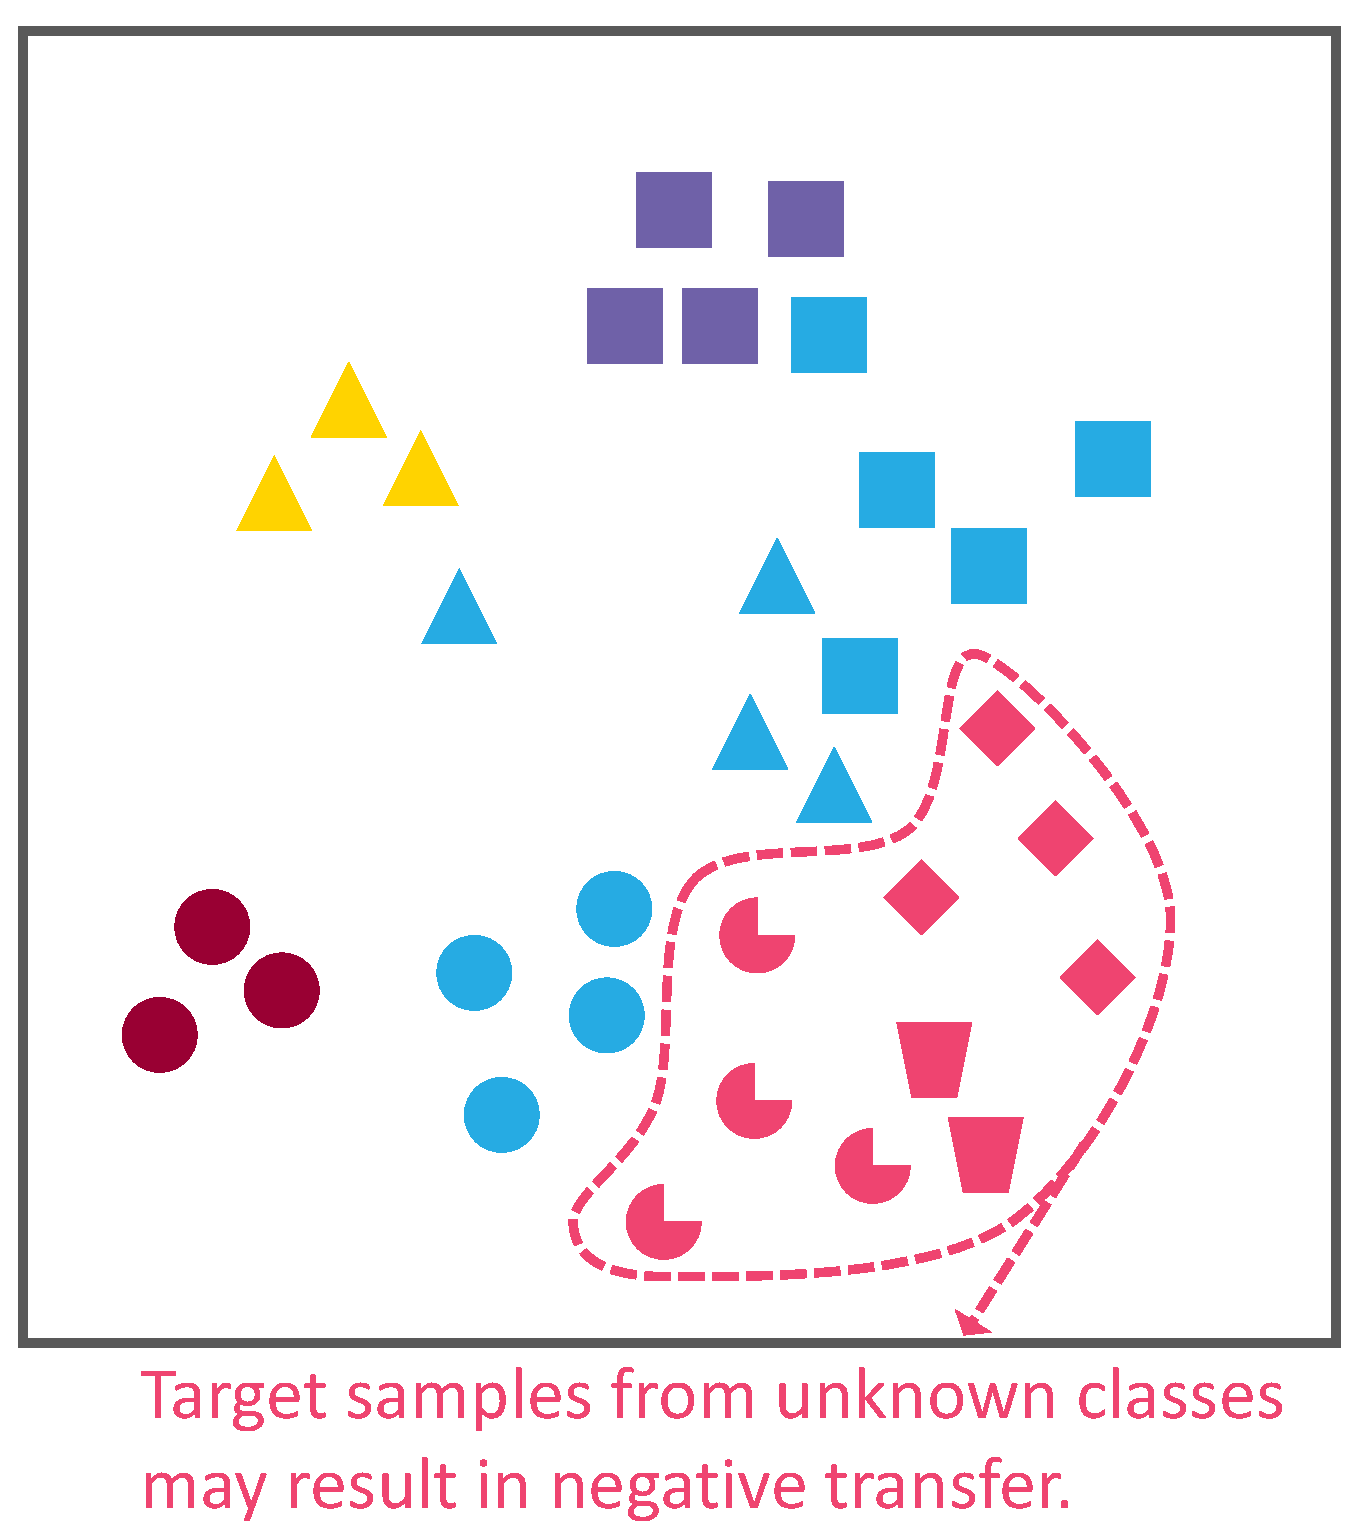
\includegraphics[width=0.22\textwidth]{contents/figures/pdf/overview/1.pdf} 
        \label{figure: reweighting based}
    } 
    \subfloat[]{
        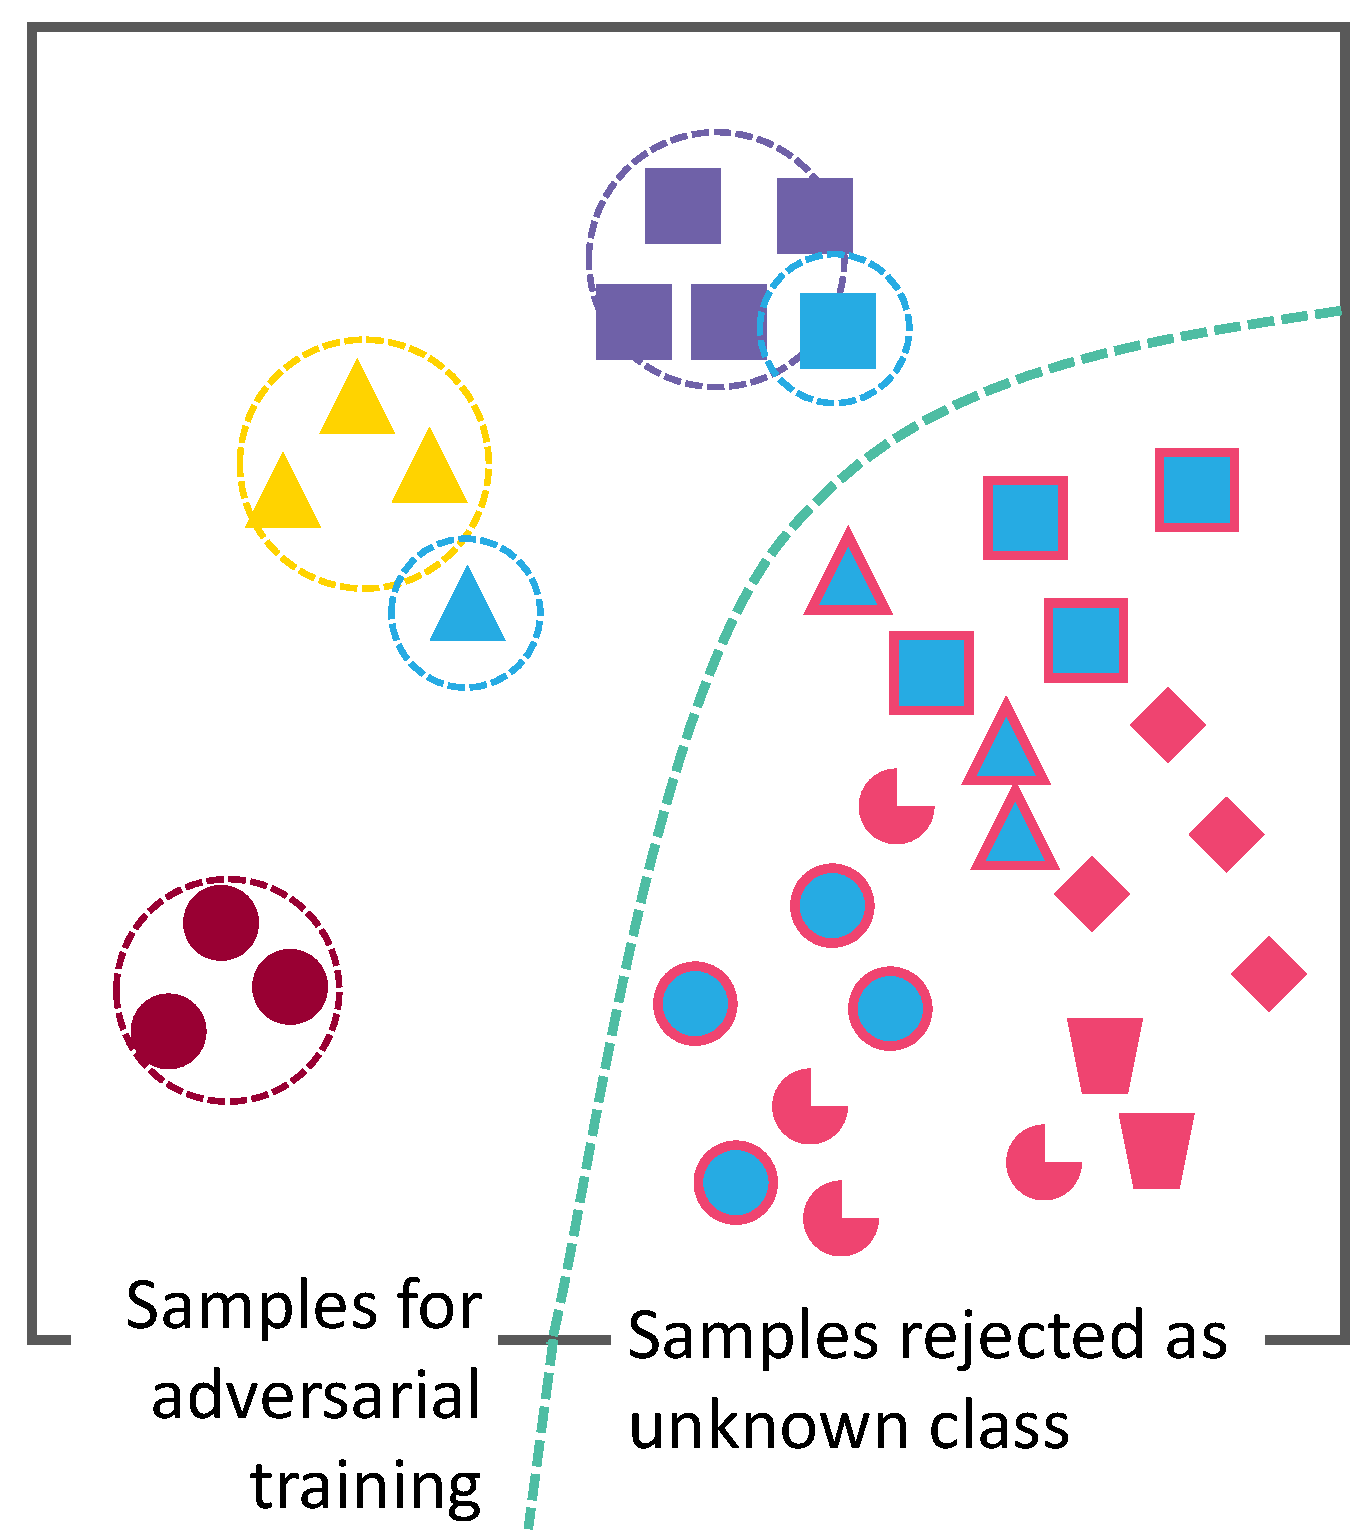
\includegraphics[width=0.22\textwidth]{contents/figures/pdf/overview/2.pdf} 
        \label{figure: ThDAN 1}
    } 
    \subfloat[]{
        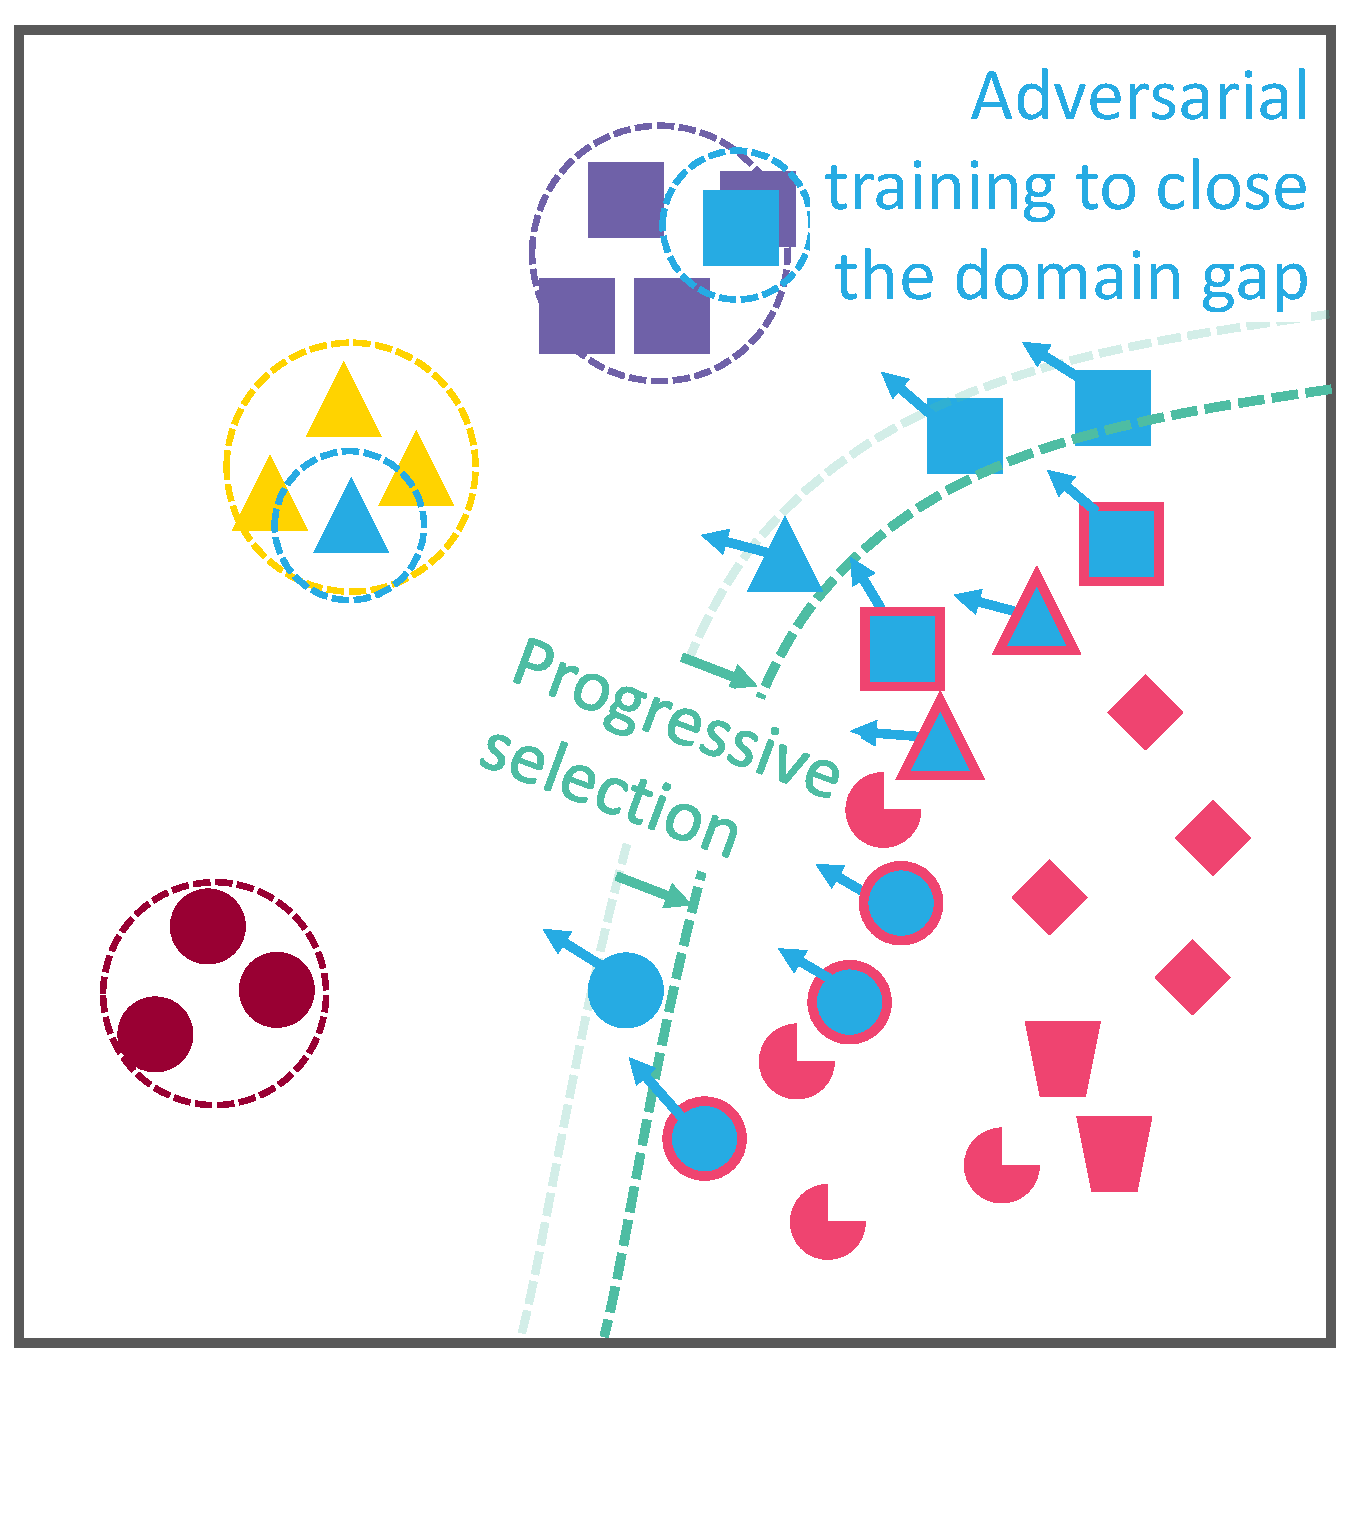
\includegraphics[width=0.22\textwidth]{contents/figures/pdf/overview/3.pdf} 
        \label{figure: ThDAN 2}
    } 
    % \hfil
    \subfloat[]{
        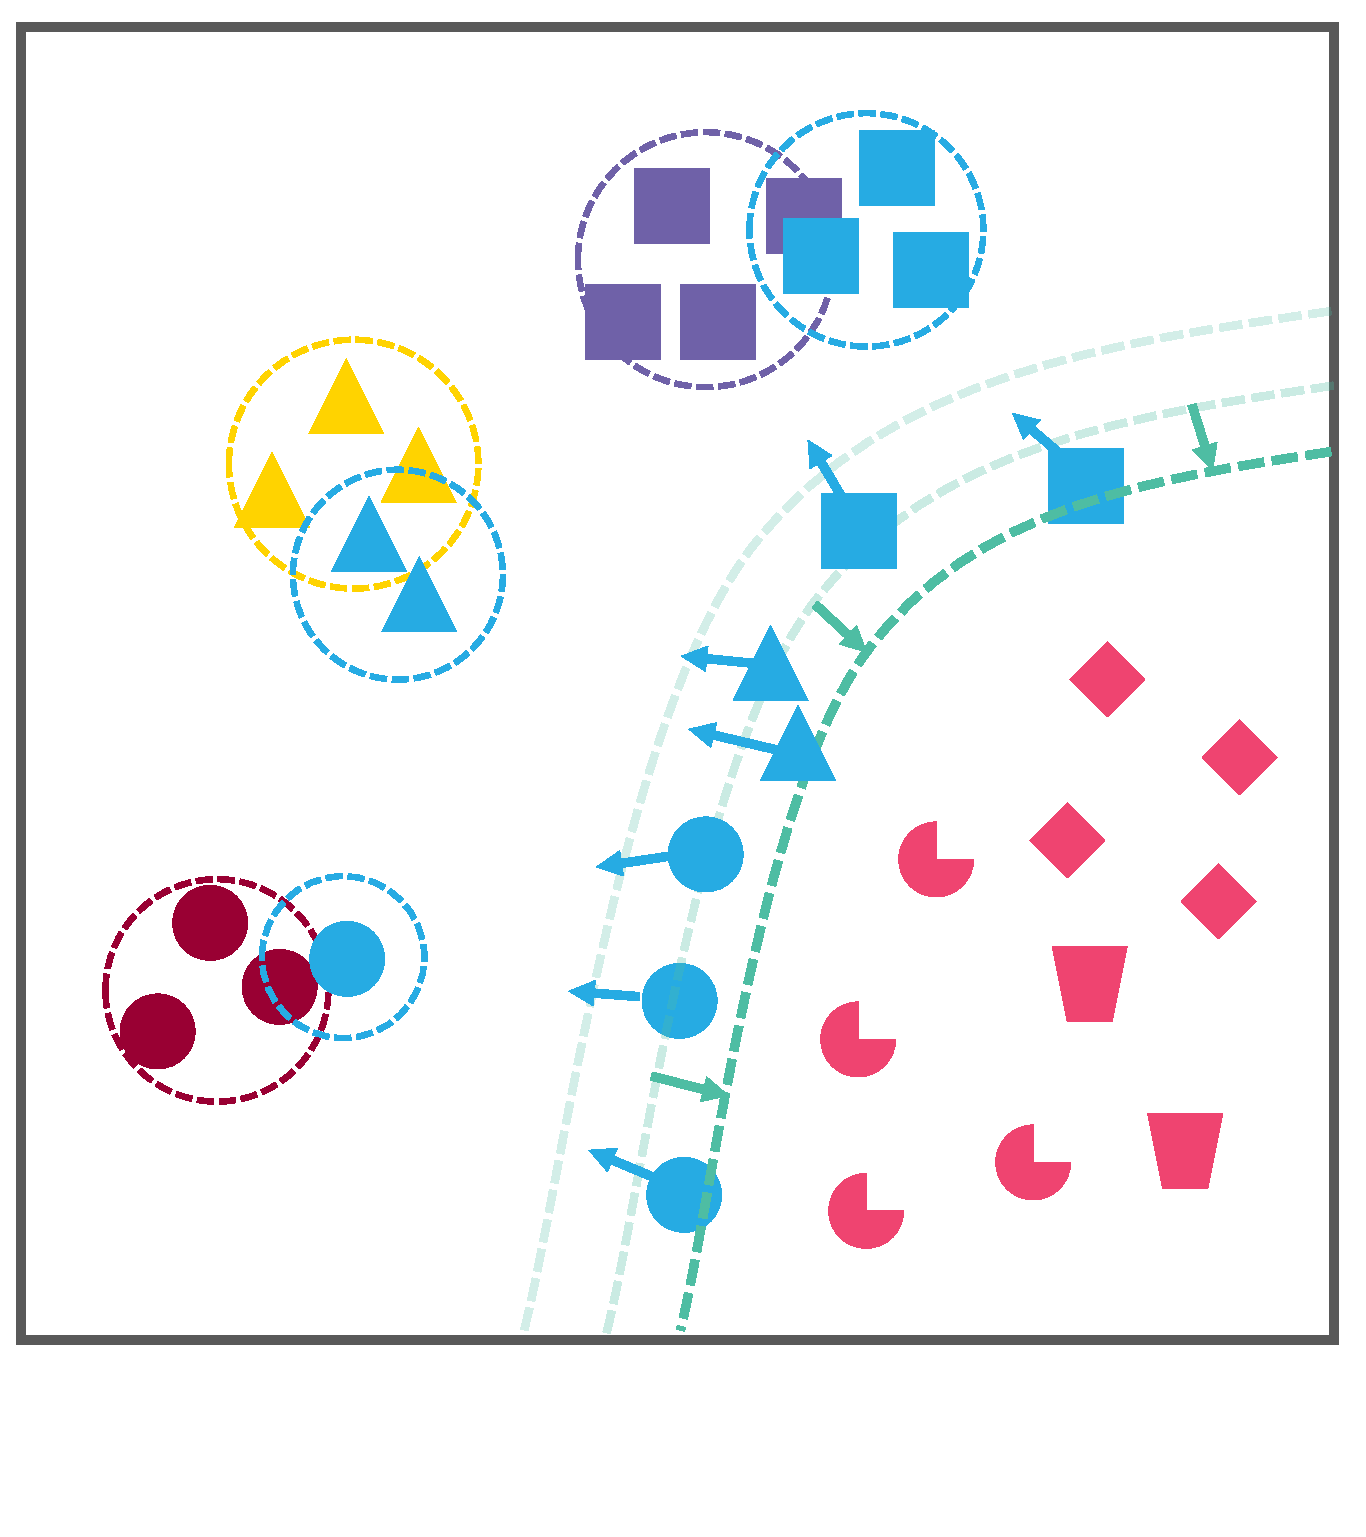
\includegraphics[width=0.22\textwidth]{contents/figures/pdf/overview/4.pdf} 
        \label{figure: ThDAN 3}
    }
    \caption{
        Figure1 of the original manuscript.
    } 
    \label{figure: overview} 
\end{figure}

